%\linespread{1.5} 
%\normalsize
This chapter contains all the simulation results and graph plots for different parameters and adequate discussion on the obtained results. All structures are simulated in wave optics module of COMSOL Multiphysics software and graphs are plotted with the help of MATLAB.

\section{HPW Structures}
We have simulated three different structures of hybrid plasmonic waveguides: InP-based deeply etched HPW, hybrid metal-insulator-metal (HMIM) plasmonic waveguide and hybrid dielectric-loaded plasmonic waveguide (HDLW). We have also studied some characteristics and properties of these structures such as propagation length and effective mode index at different widths and thicknesses of the waveguides.

\subsection{Silicon-based HPW with Metal Cap}
The simulation results of HPW structure discussed in Section~\ref{subsubsec:nslc_shpw} are shown in this section. Fig.~\ref{fig:nslc_mode_profile} shows the field distribution of the major-component $E_\text{y}$ of the electrical fields. From these figures, one sees that there is more optical confinement in the Si layer when the core width increases. This is why the effective index real($n_\text{eff}$) and the propagation distance $L_\text{prop}$ increases as the core width increases, as shown in Fig.~\ref{fig:nslc_neffr} and ~\ref{fig:nslc_proplen}, respectively. We also see that the thickness $h_\text{SiO2}$ of the $\text{SiO}_2$ nano-layer plays an important role for the propagation distance. When choosing a thinner $\text{SiO}_2$ layer, the propagation distance becomes smaller. For the case with a relatively large thickness $h_\text{SiO2}$ (e.g., 50 nm), more power confined in silicon region. Therefore, when the core width decreases, the power confined in the silicon region will change greatly. This is why the influence of the core width on the propagation distances is significant when the thickness $h_\text{SiO2}$ is relatively large.

\begin{figure}[!t]
	\centering
	\includegraphics[width=1\textwidth]{shpw_mc_mode.jpg}
	\caption{Field distribution of the major component $E_\text{y}$ of the quasi-TM fundamental mode for the cases of $w_\text{co}$ = 100nm, 300nm, and 500nm.}
	\label{fig:nslc_mode_profile}
\end{figure}

\begin{figure}[!t]
	\centering
	\includegraphics[width=1\textwidth]{nslc_neffr_eps}
	\caption{The real part of the effective refractive index $n_\text{eff}$ for $h_\text{SiO2}$ = 5nm, 20nm, and 50nm.}
	\label{fig:nslc_neffr}
\end{figure}

\begin{figure}[!t]
	\centering
	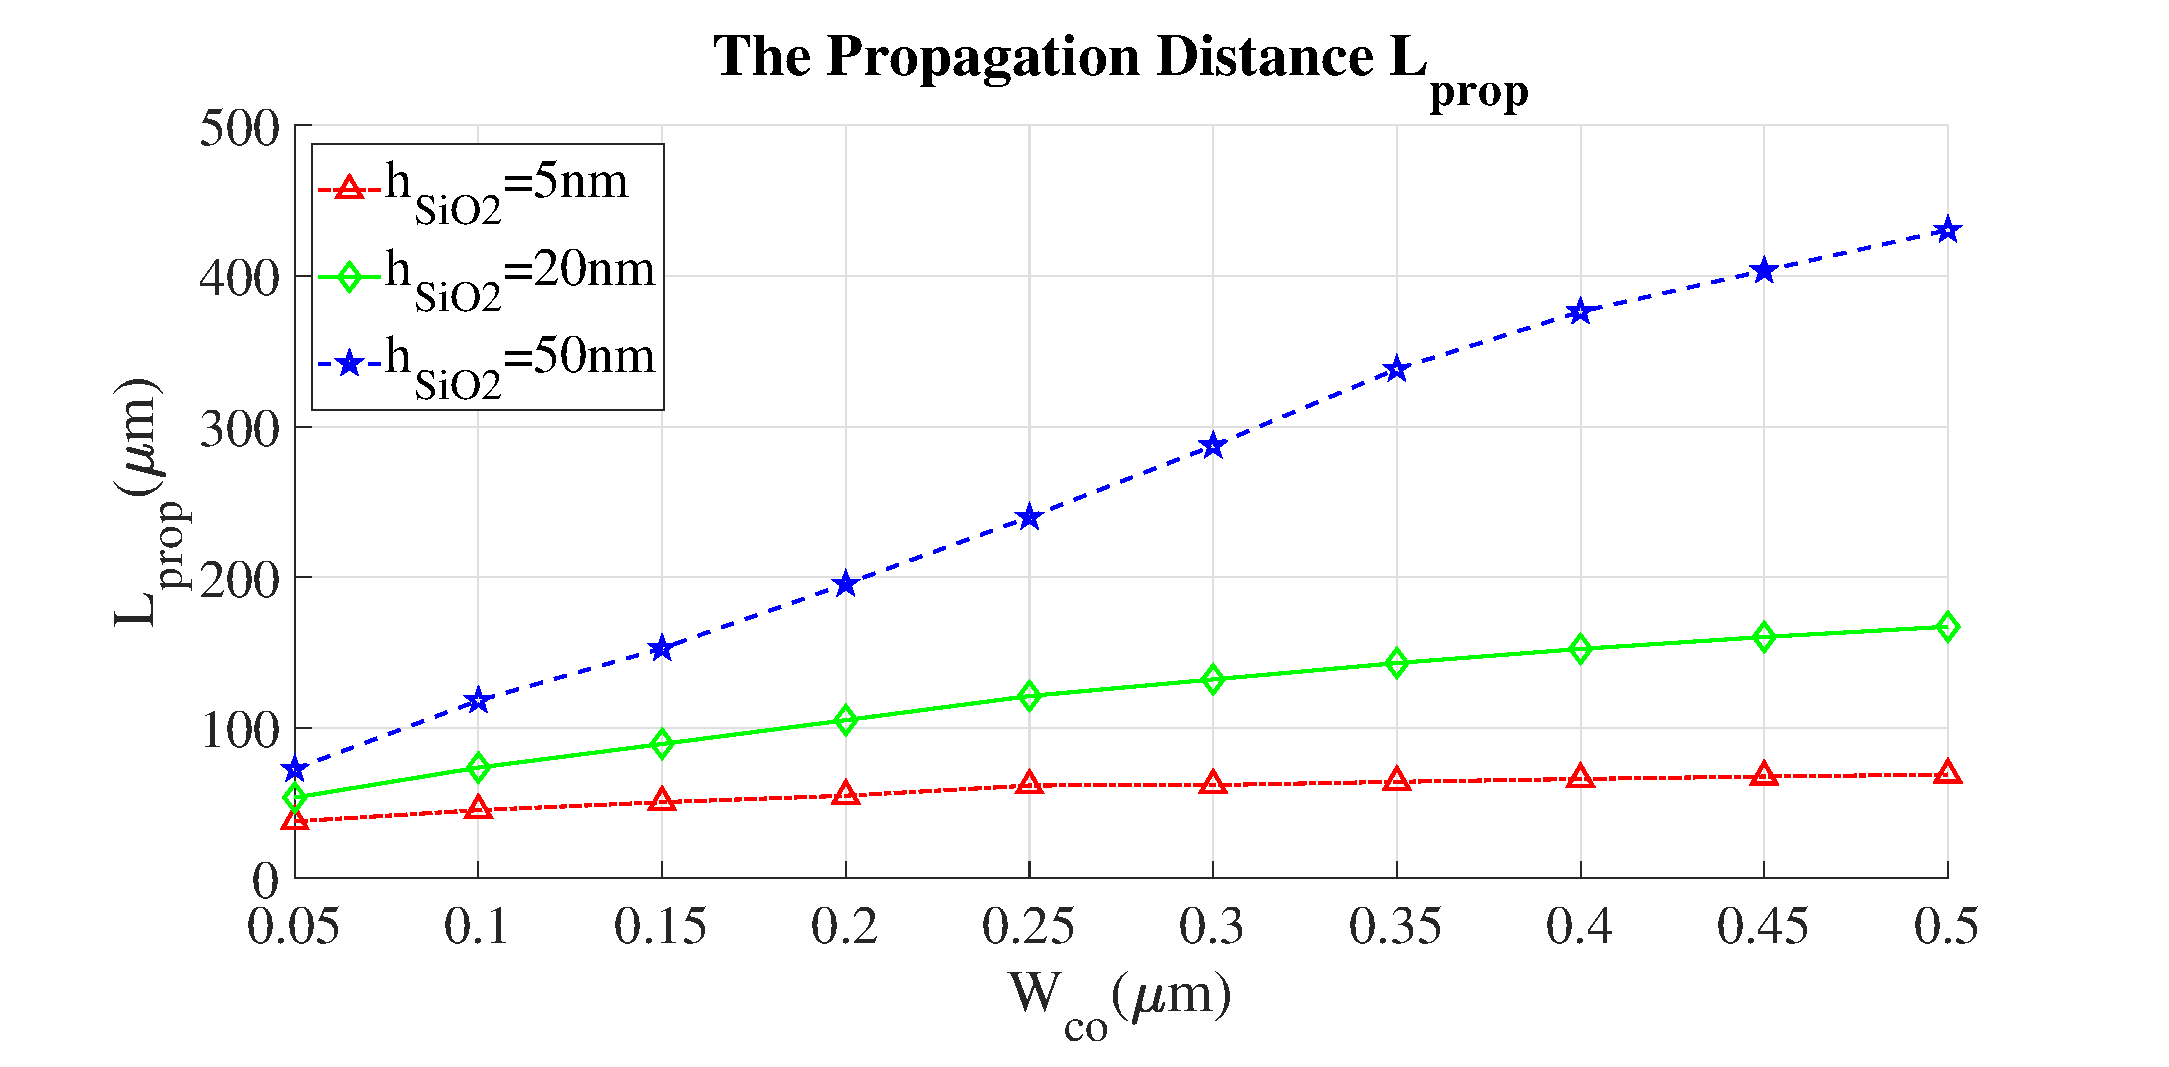
\includegraphics[width=1\textwidth]{nslc_proplen_eps}
	\caption{The propagation length $L_\text{prop}$ for $h_\text{SiO2}$ = 5nm, 20nm, and 50nm.}
	\label{fig:nslc_proplen}
\end{figure}

In summary, the calculation results in Fig.~\ref{fig:nslc_neffr} and ~\ref{fig:nslc_proplen} show that the present hybrid plasmonic waveguide supports a propagation distance on the order of several tens of wavelength $\uplambda$, which is useful to develop plasmonic waveguide devices. One should note that there is a trade-off between the dimension of the plasmon waveguide and its propagation distance.

\subsection{HMIM Plasmonic Waveguide}
The simulation results of the HMIM multilayered plasmonic waveguide described in the Section~\ref{subsubsec:hmim_pw} are shown in here. Mode is confined in both spacer layers.

Fig.~\ref{fig:hmim-neffr} and ~\ref{fig:hmim-neffi} contain the real and imaginary part of the effective mode index of HMIM waveguide for different thickness of spacer and high-dielectric layers respectively. Fig.~\ref{fig:hmim-proplen} shows the propagation length plot of HMIM waveguide for different spacer and high-dielectric layer thickness. Maximum propagation length of 260$\upmu \text{m}$ has been observed at t\_h=300nm, t\_s=200nm.

\begin{figure}[!t]
	\centering
	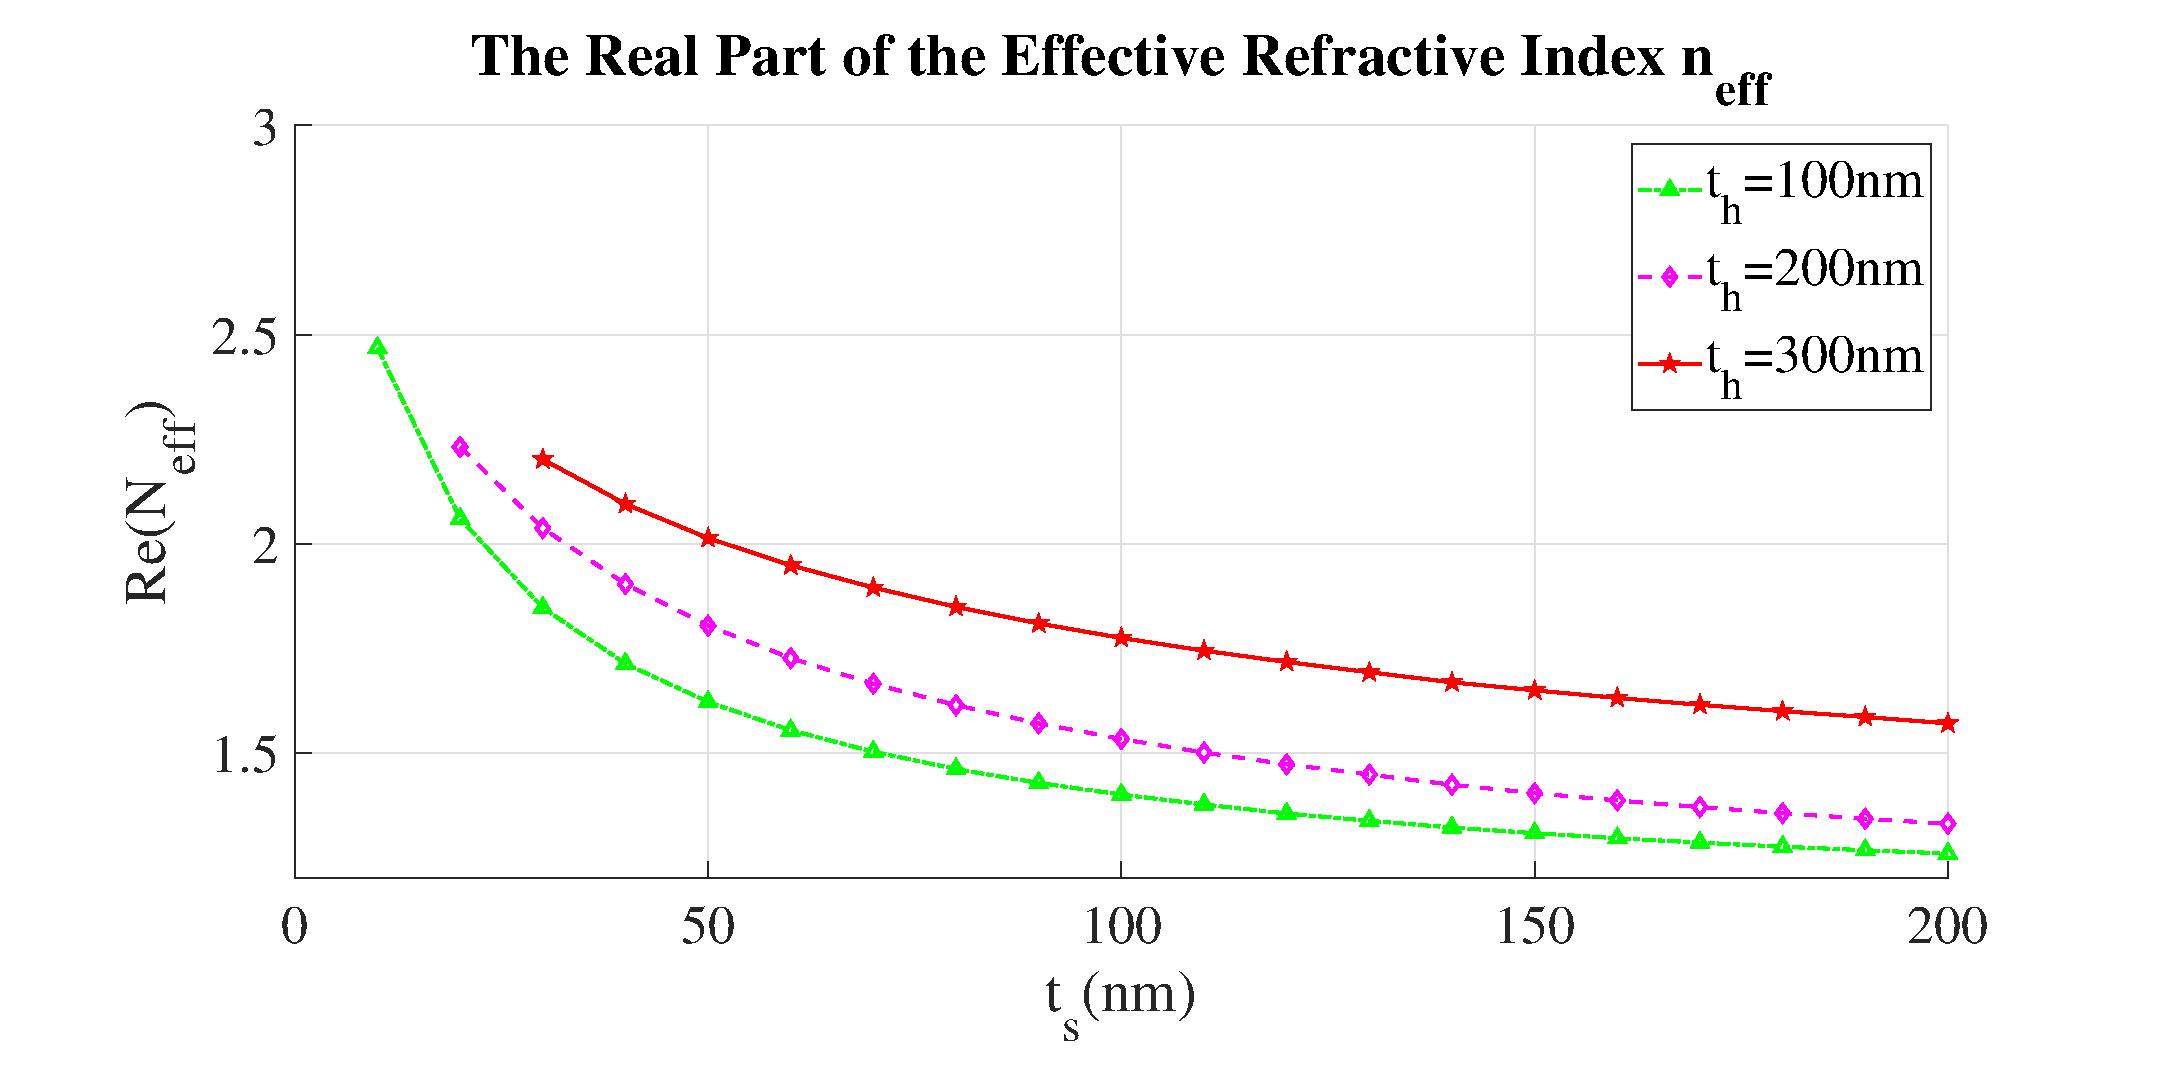
\includegraphics[width=1\textwidth]{hmim-neffr-eps}
	\caption{Real part of effective mode index of hybrid metal insulator metal (HMIM) waveguide.}
	\label{fig:hmim-neffr}
\end{figure}

\begin{figure}[!t]
	\centering
	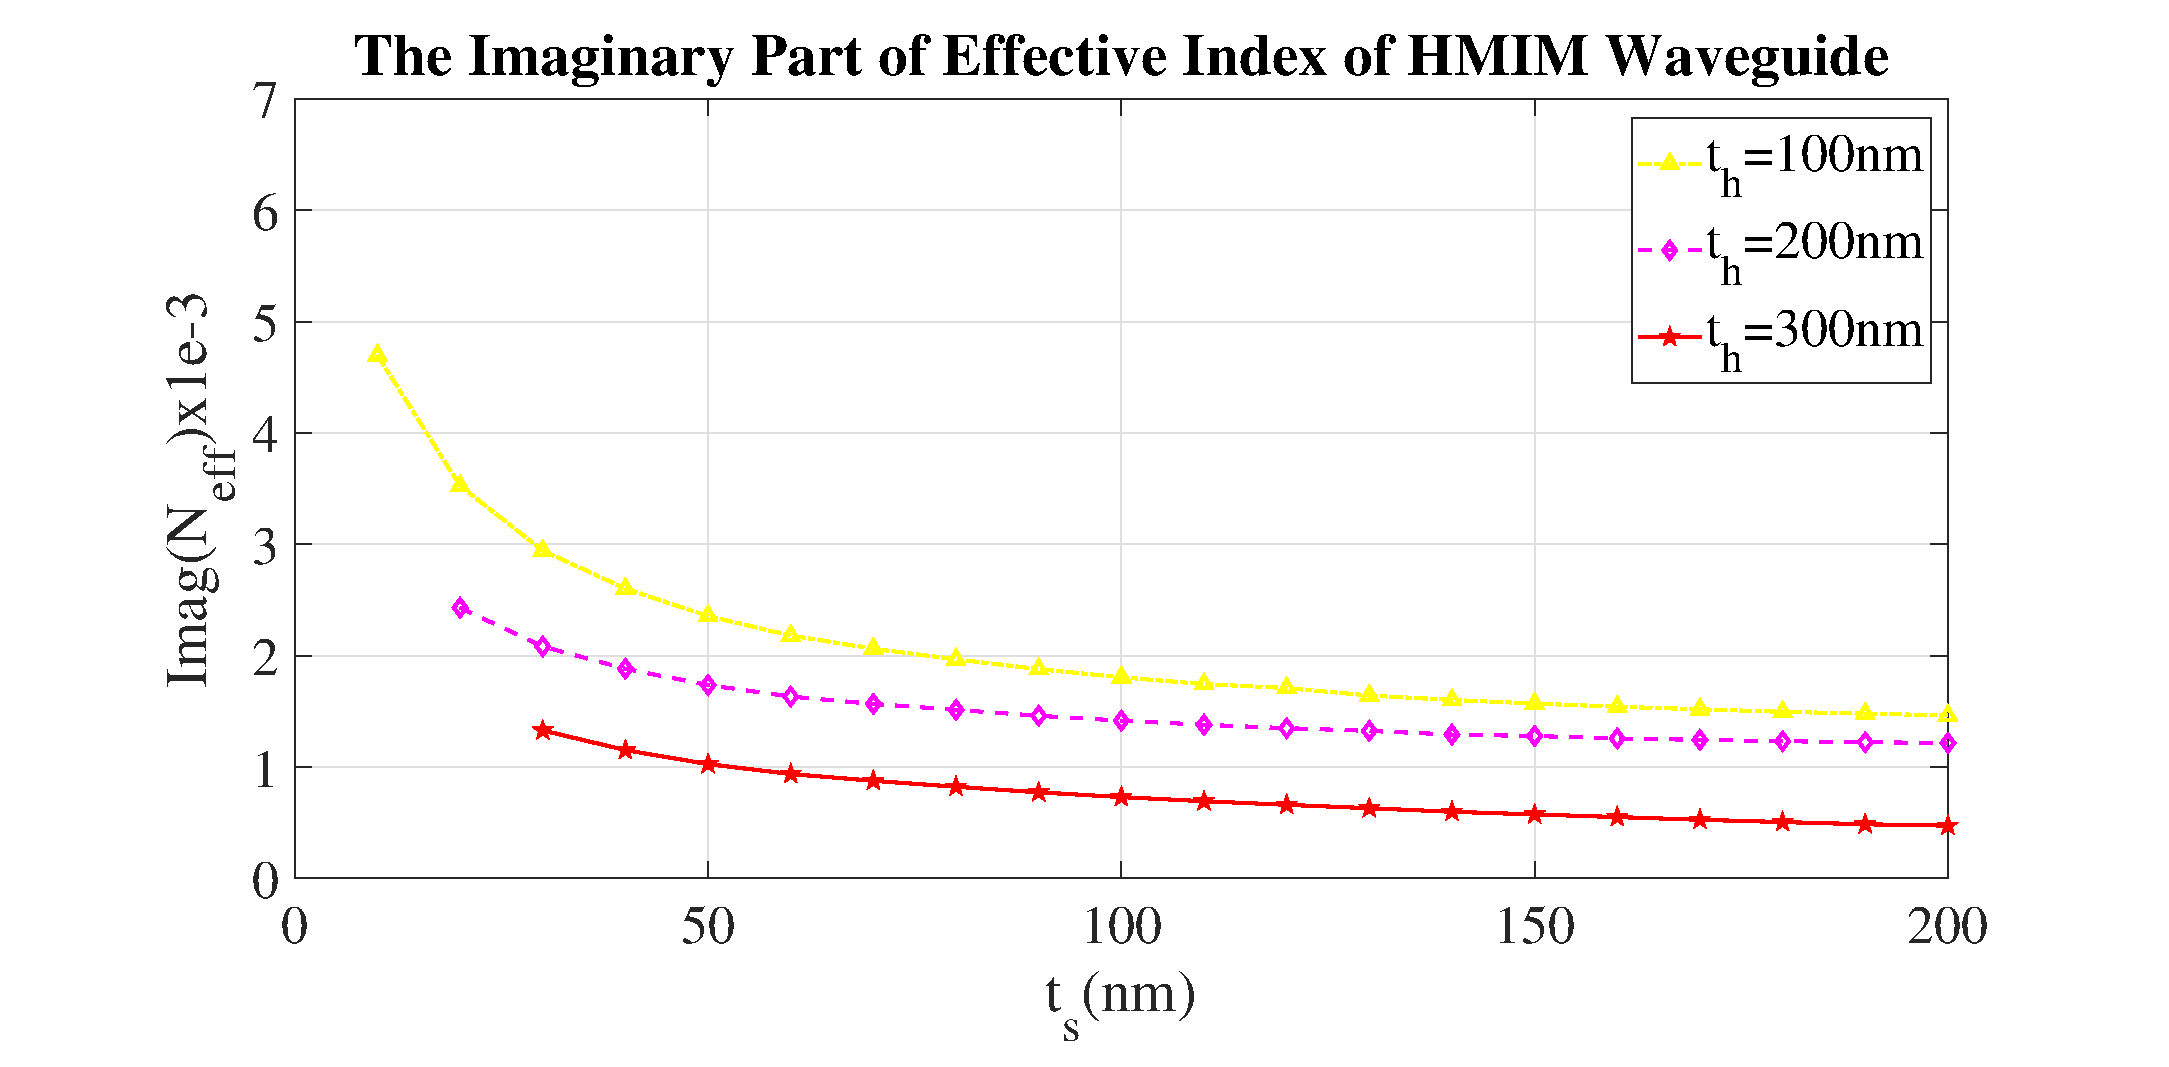
\includegraphics[width=1\textwidth]{hmim-neffi-eps}
	\caption{Imaginary part of effective mode index of hybrid metal insulator metal (HMIM) waveguide.}
	\label{fig:hmim-neffi}
\end{figure}

\begin{figure}[!t]
	\centering
	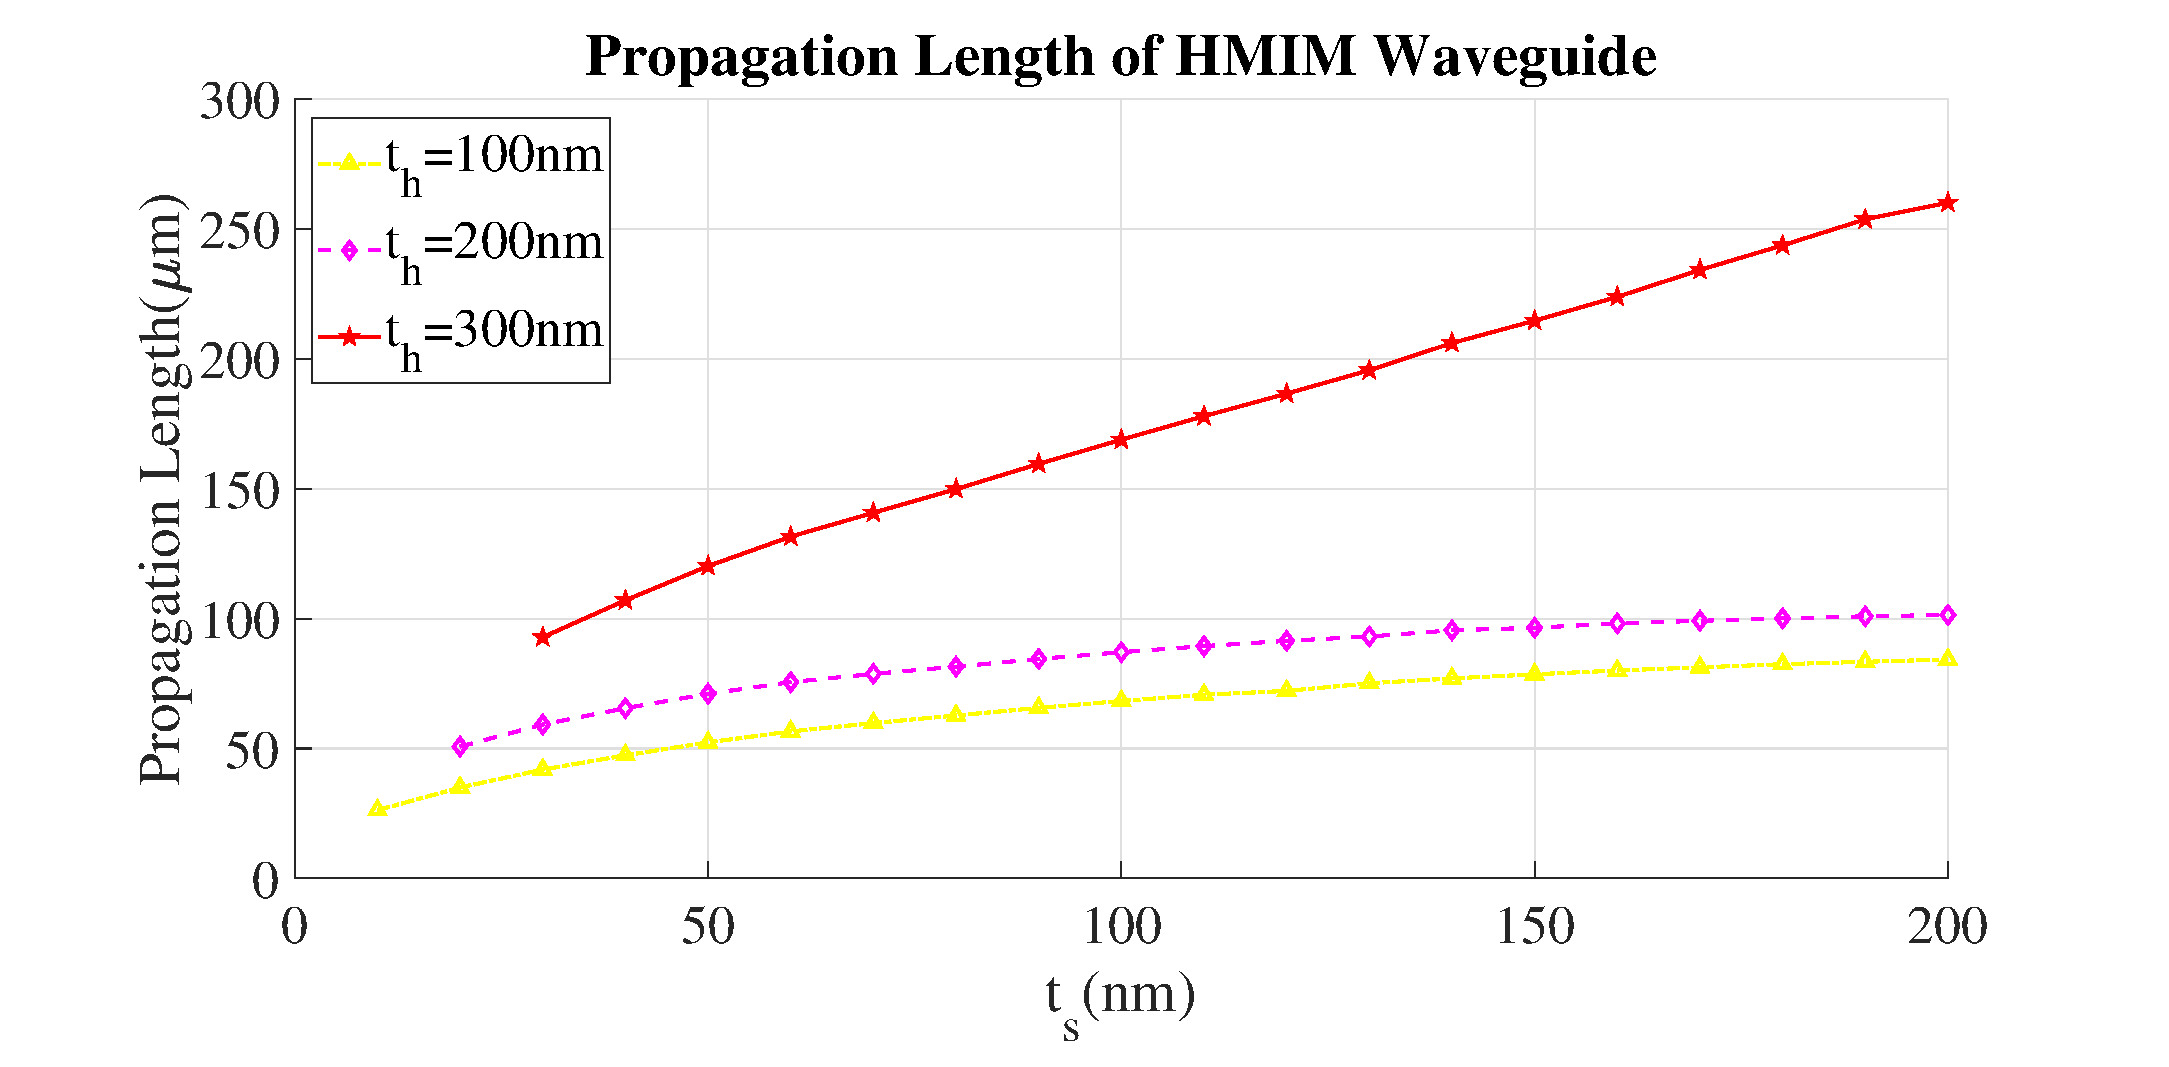
\includegraphics[width=1\textwidth]{hmim-proplen-eps}
	\caption{Propagation length of hybrid metal insulator metal (HMIM) waveguide.}
	\label{fig:hmim-proplen}
\end{figure}

\subsection{InP-based HP-Waveguide}
The InP-based deeply etched hybrid plasmonic waveguide consists of an InGaAsP core layer with a thickness of 500 nm and a bandgap energy of 0.992 eV (equal to a bandgap wavelength of 1.25 $\mu$m) denoted as Q(1.25), an InP cladding layer with a thickness of 160 nm on a semi-insulating InP substrate. The layer stack of hybrid plasmonic waveguide is capped by gold (Au) or silver (Ag) with a thickness of 110 nm. The thickness of the capped metal is optimized during the simulation of passive devices to enhance the power transmission from an input waveguides into the output waveguide. The refractive index of InGaAsP (Q(1.25)), InP, and gold (Au) are equal to 3.3636, 3.1669, and 0.187 + 10.3457i, respectively, at a wavelength of 1550 nm~\cite{Nikoufard2017}.

Mode profile of InP-based HP-waveguide is shown in Fig.~\ref{fig:InP_hpw_modeprofile}. Fig.~\ref{fig:MMI_neffr} shows the real part of effective refractive index of the first five TM modes at the wavelength of 1.55 $\mu$m for the HP-waveguide. In the HP-waveguide, the fundamental $\text{TM}_{00}$ mode does not exhibit a cutoff, and the number of modes supported by the HP-waveguide increases with the width of the ridge. The cutoff widths for $\text{TM}_{01}$, $\text{TM}_{02}$, and $\text{TM}_{03}$ modes are equal to 400, 700, and 1200 nm, respectively. The real part of the effective refractive index approaches toward the refractive index of the InGaAsP layer, as the width of the ridge increases.

\begin{figure}[!t]
	\centering
	\includegraphics[width=0.5\textwidth,height=0.3\textheight]{InP_hpw_mode}
	\caption{Mode profile of InP-based HP-waveguide.}
	\label{fig:InP_hpw_modeprofile}
\end{figure}

\begin{figure}[!t]
	\centering
	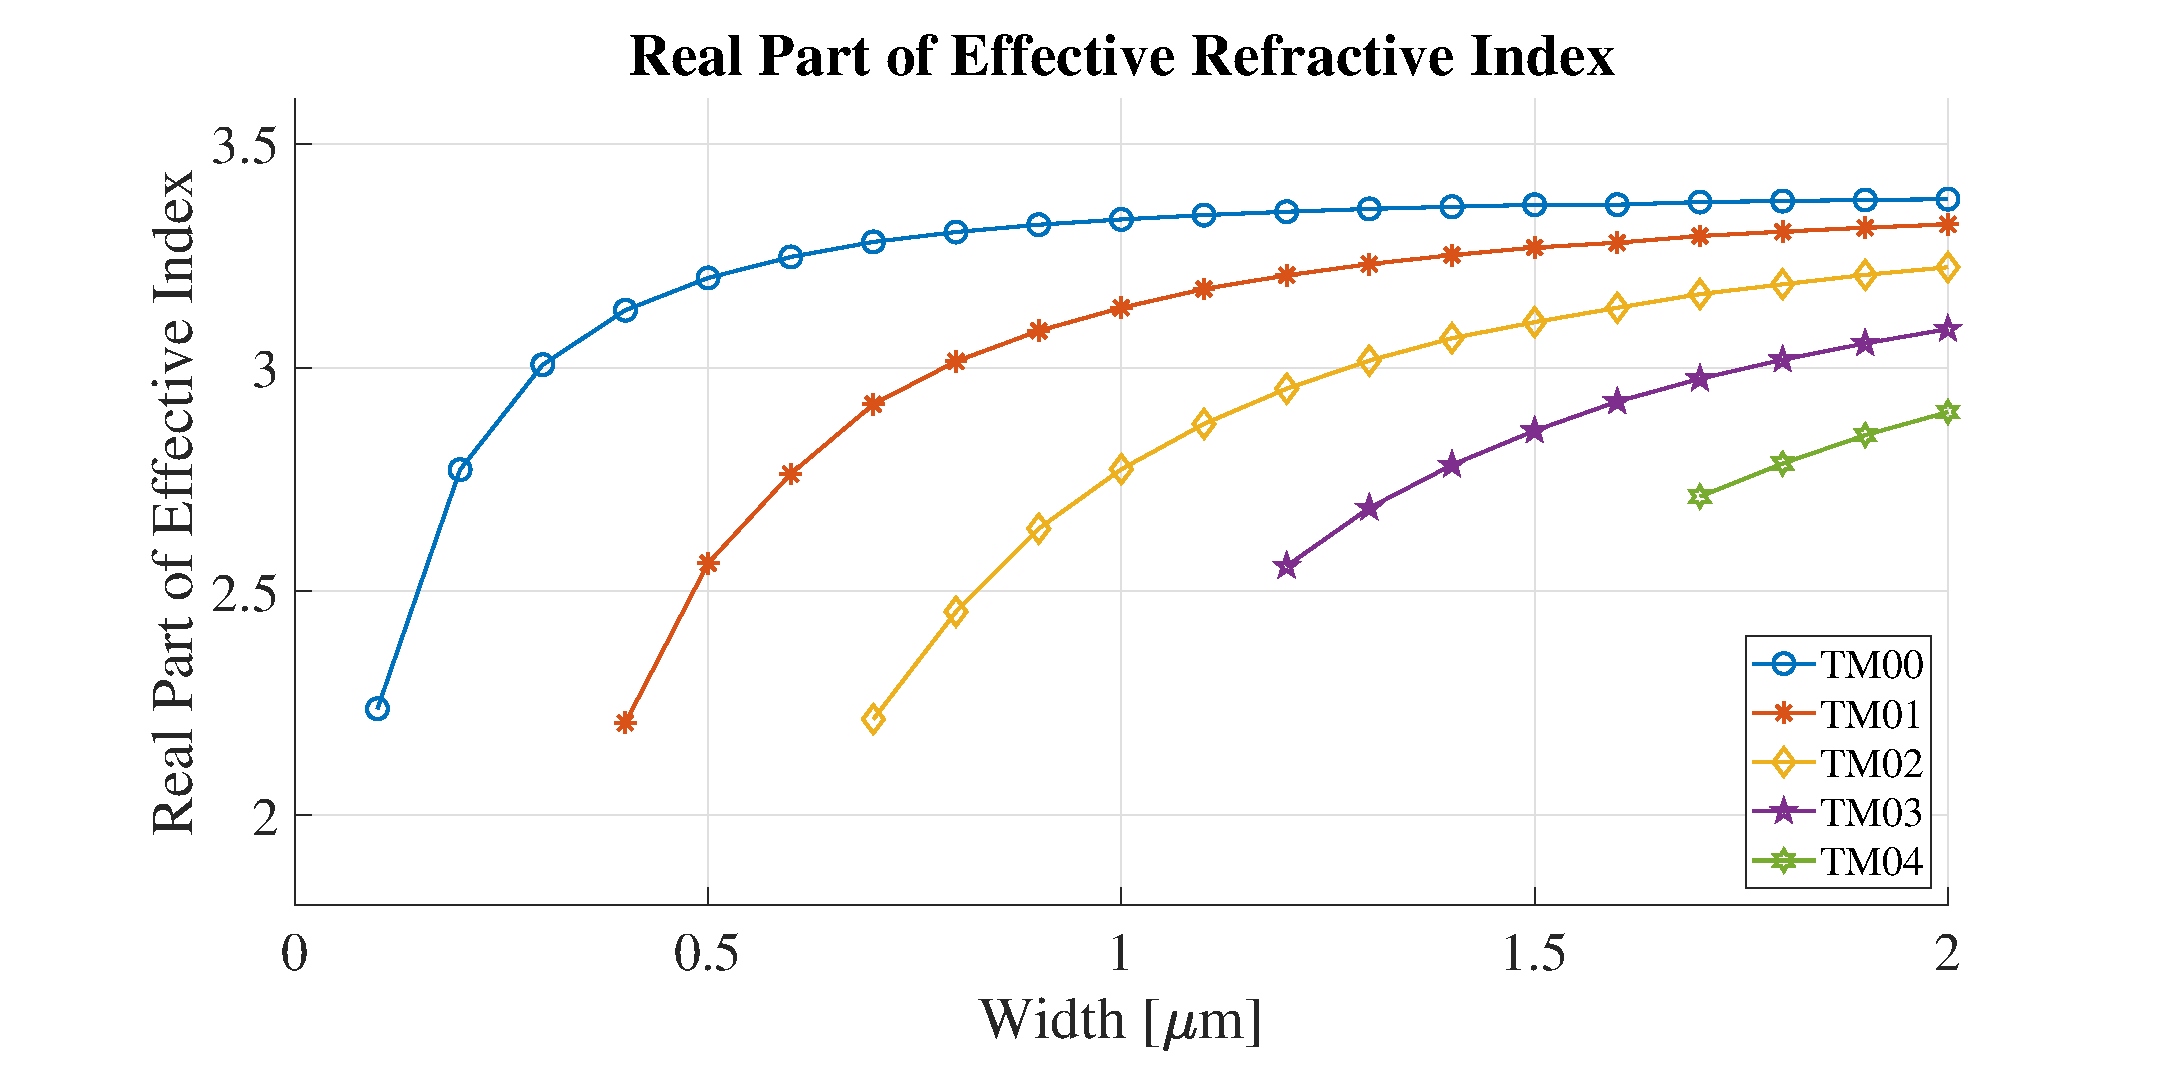
\includegraphics[width=1\textwidth]{MMI_neffr_eps}
	\caption{Real part of effective refractive index for fundamental ($\text{TM}_{00}$), first ($\text{TM}_{01}$), second ($\text{TM}_{02}$), third ($\text{TM}_{03}$), and fourth ($\text{TM}_{04}$) modes, as a function of the width of InP-based HP-waveguide.}
	\label{fig:MMI_neffr}
\end{figure}

\begin{figure}[!t]
	\centering
	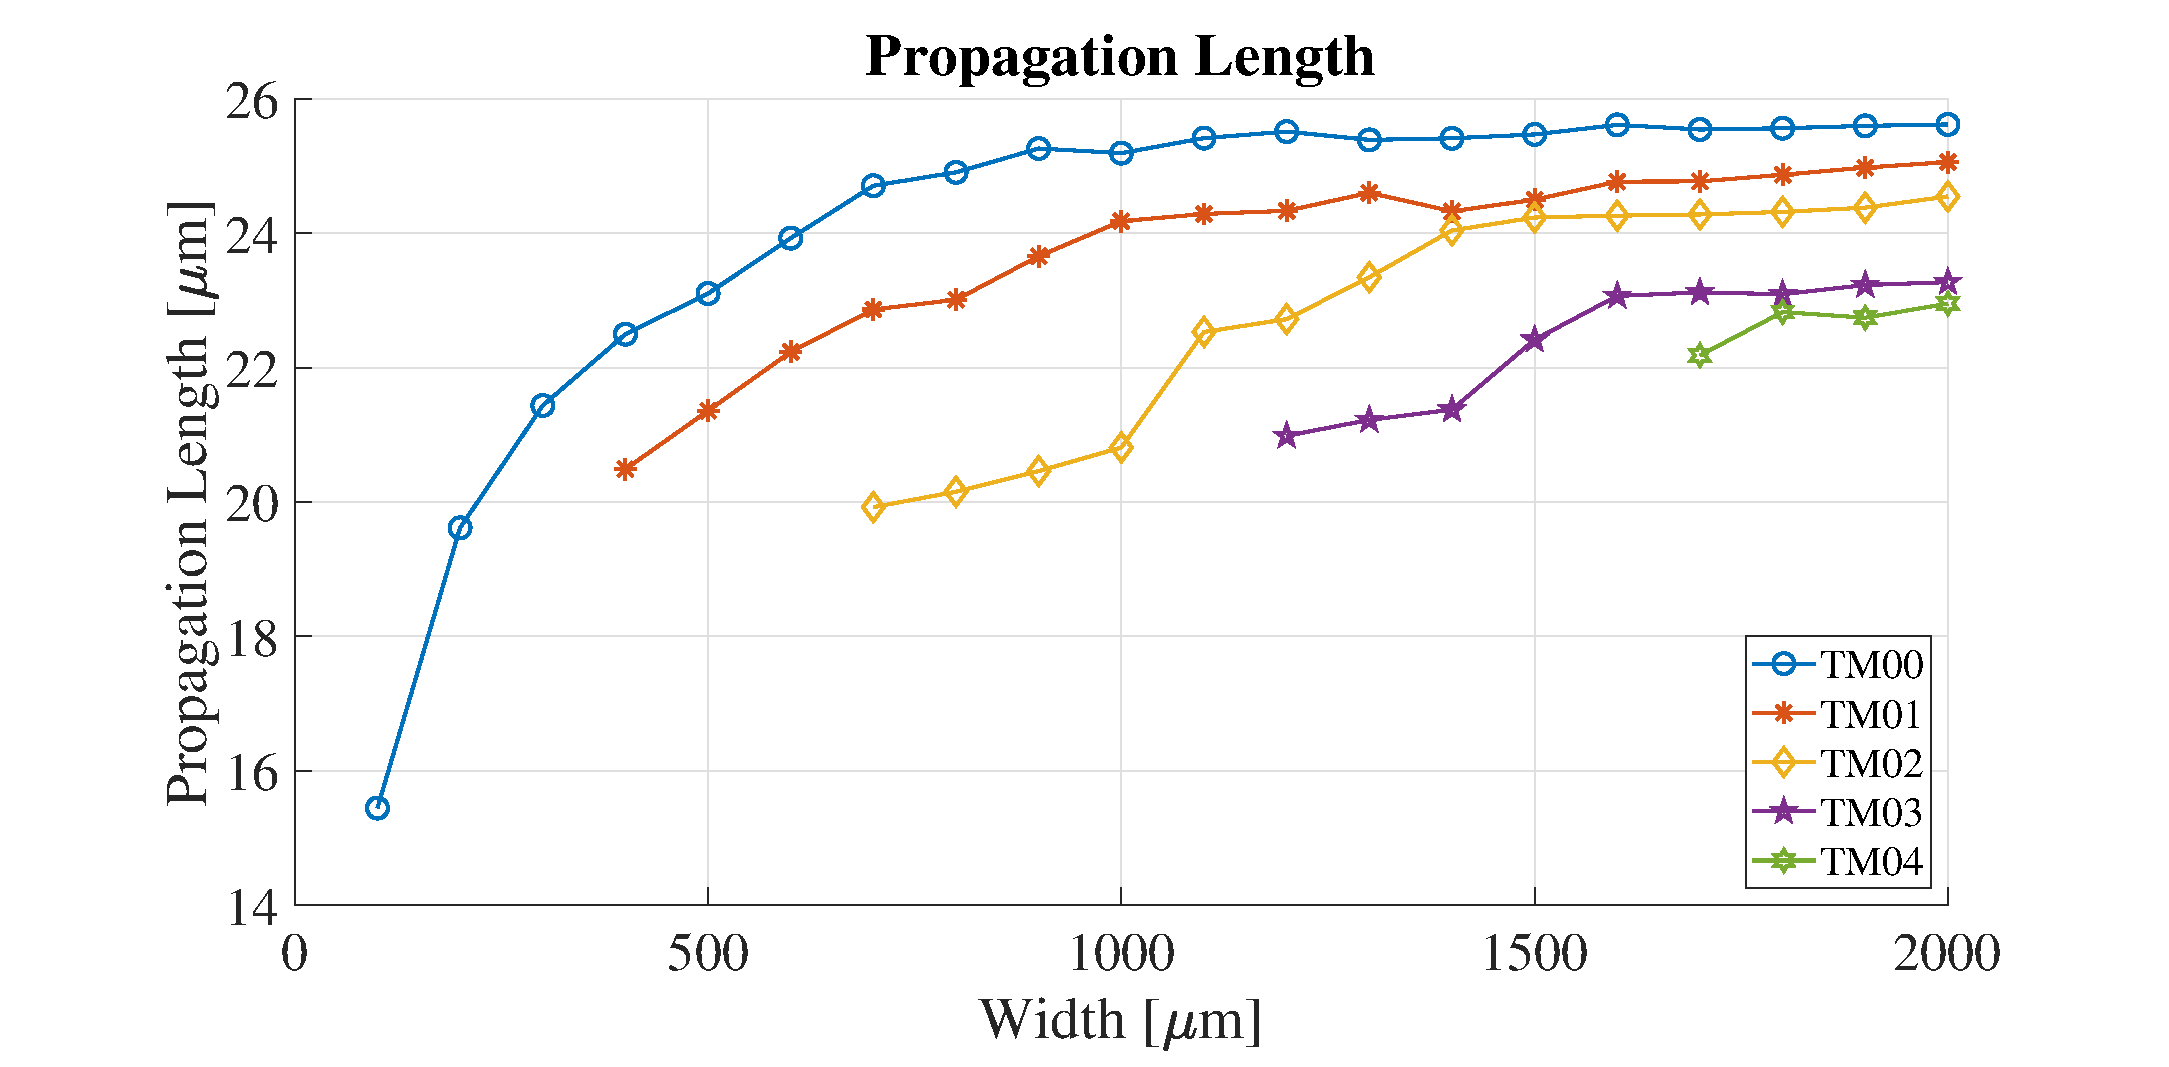
\includegraphics[width=1\textwidth]{MMI_proplen_eps}
	\caption{Propagation length as a function of the InP-based HP-waveguide for $\text{TM}_{00}$, $\text{TM}_{01}$, $\text{TM}_{02}$, $\text{TM}_{03}$, and $\text{TM}_{04}$ modes, determined from the imaginary part of the effective refractive index.}
	\label{fig:MMI_proplen}
\end{figure}

The propagation length of the deeply etched HP-waveguide, determined from the imaginary part of the effective refractive index, i.e., $L_\text{p}$ = $1/(2k_0 n_{\text{eff,imag}})$, where $n_{\text{eff,imag}}$ is the imaginary part of the effective refractive index of the HP waveguide and $k_0 = 2\pi/ \lambda$ is the wavenumber in vacuum. The propagation length for first five TM modes at the wavelength of 1.55 $\mu$m is show in Fig.~\ref{fig:MMI_proplen}.

\section{HPW Devices}
In this section, we present the simulation result of optical ring resonator (ORR) based on  hybrid dielectric-loaded plasmonic waveguide (HDLW). We also discuss the characteristics of SOI-based hybrid plasmonic waveguide horn nanoantenna.

\subsection{Ring Resonator}
Fig.~\ref{fig:hdlw_efield_2000nm_res} and ~\ref{fig:hdlw_efield_2000nm_non_res} show the E-field norm distribution of HDLW-based ring resonator at R = 2000nm for both resonating and non-resonating wavelengths respectively. While, Fig.~\ref{fig:hdlw_efield_5000nm_res} and ~\ref{fig:hdlw_efield_5000nm_non_res} show the E-field norm distribution of HDLW-based ring resonator at R = 5000nm for both resonating and non-resonating wavelengths respectively.  It is clear from the figure that whenever phase is integral multiple of 2$\uppi$, almost entire power is coupled in the ring waveguide and a very negligible amount of power is transmitted at output port. This explains the properties of notch filter i.e., for a range of frequencies, there is a very negligible amount of power transmitted at the output port and most of the power is coupled in the ring waveguide.

The transmission characteristics of ring resonator are shown in the Fig.~\ref{fig:hdlw_transmission}. As it can be seen from the figure that extinction ratio is relatively higher when R = 5 $\upmu\text{m}$ as compared to that of R = 2 $\upmu\text{m}$. This explains the fact that in order to get better (smaller) confinement, we have to trade-off between propagation loss and the confinement area. The values of some important parameters for the simulation of this resonator structure are listed in the table~\ref{tab:rr_params}. These parameters can be changed as per requirement.

\renewcommand{\arraystretch}{1.3}
\begin{table}[!t]
	\begin{center}
		\caption{\label{tab:rr_params} Design Parameters of Ring Resonator.}%\vspace{-2.0mm}
		\scalebox{0.95}{
			\begin{tabular}{ccc}\hline
				Parameter 	&	Value	&	Description\\ \hline 
				R 			& 2 or 5 $\upmu\text{m}$ & Ring radius\\ \hline 
				g 			& 200 or 150 nm & Gap distance\\ \hline
				t$_{\text{SiO}_2}$	& 50 nm & $\text{SiO}_2$ thickness\\ \hline
				t$_{\text{Si}}$	& 150 nm & Si thickness\\ \hline
				t$_{\text{Ag}}$	& 100 nm & Ag thickness\\ \hline
				W			& 300 nm & Waveguide width\\ \hline
				N$_{\text{Si}}$ & 3.4785 & Si refractive index\\ \hline
				N$_{\text{SiO}_2}$	& 1.4491 & $\text{SiO}_2$ refractive index\\ \hline
				N$_{\text{Ag}}$ & 0.1453 +11.3587i & Ag refractive index\\ \hline
			\end{tabular}
		}%\vspace{-3mm}
	\end{center}
\end{table}

\begin{figure}[!t]
	\centering
	\includegraphics[width=1\textwidth]{hdlw_normE_dist_2000nm_res}
	\caption{E-field norm distribution of HDLW based ring resonator at resonating wavelength $(\lambda = 1.58 \mu m)$.}
	\label{fig:hdlw_efield_2000nm_res}
\end{figure}

\begin{figure}[!t]
	\centering
	\includegraphics[width=1\textwidth]{hdlw_normE_dist_2000nm_non_res}
	\caption{E-field norm distribution of HDLW based ring resonator at non-resonating wavelength $(\lambda = 1.60 \mu m)$.}
	\label{fig:hdlw_efield_2000nm_non_res}
\end{figure}

\begin{figure}[!t]
	\centering
	\includegraphics[width=1\textwidth]{hdlw_normE_dist_5000nm_res}
	\caption{E-field norm distribution of HDLW based ring resonator at resonating wavelength $(\lambda = 1.592 \mu m)$.}
	\label{fig:hdlw_efield_5000nm_res}
\end{figure}

\begin{figure}[!t]
	\centering
	\includegraphics[width=1\textwidth]{hdlw_normE_dist_5000nm_non_res}
	\caption{E-field norm distribution of HDLW based ring resonator at non-resonating wavelength $(\lambda = 1.58 \mu m)$.}
	\label{fig:hdlw_efield_5000nm_non_res}
\end{figure}

\begin{figure}[!t]
	\centering
	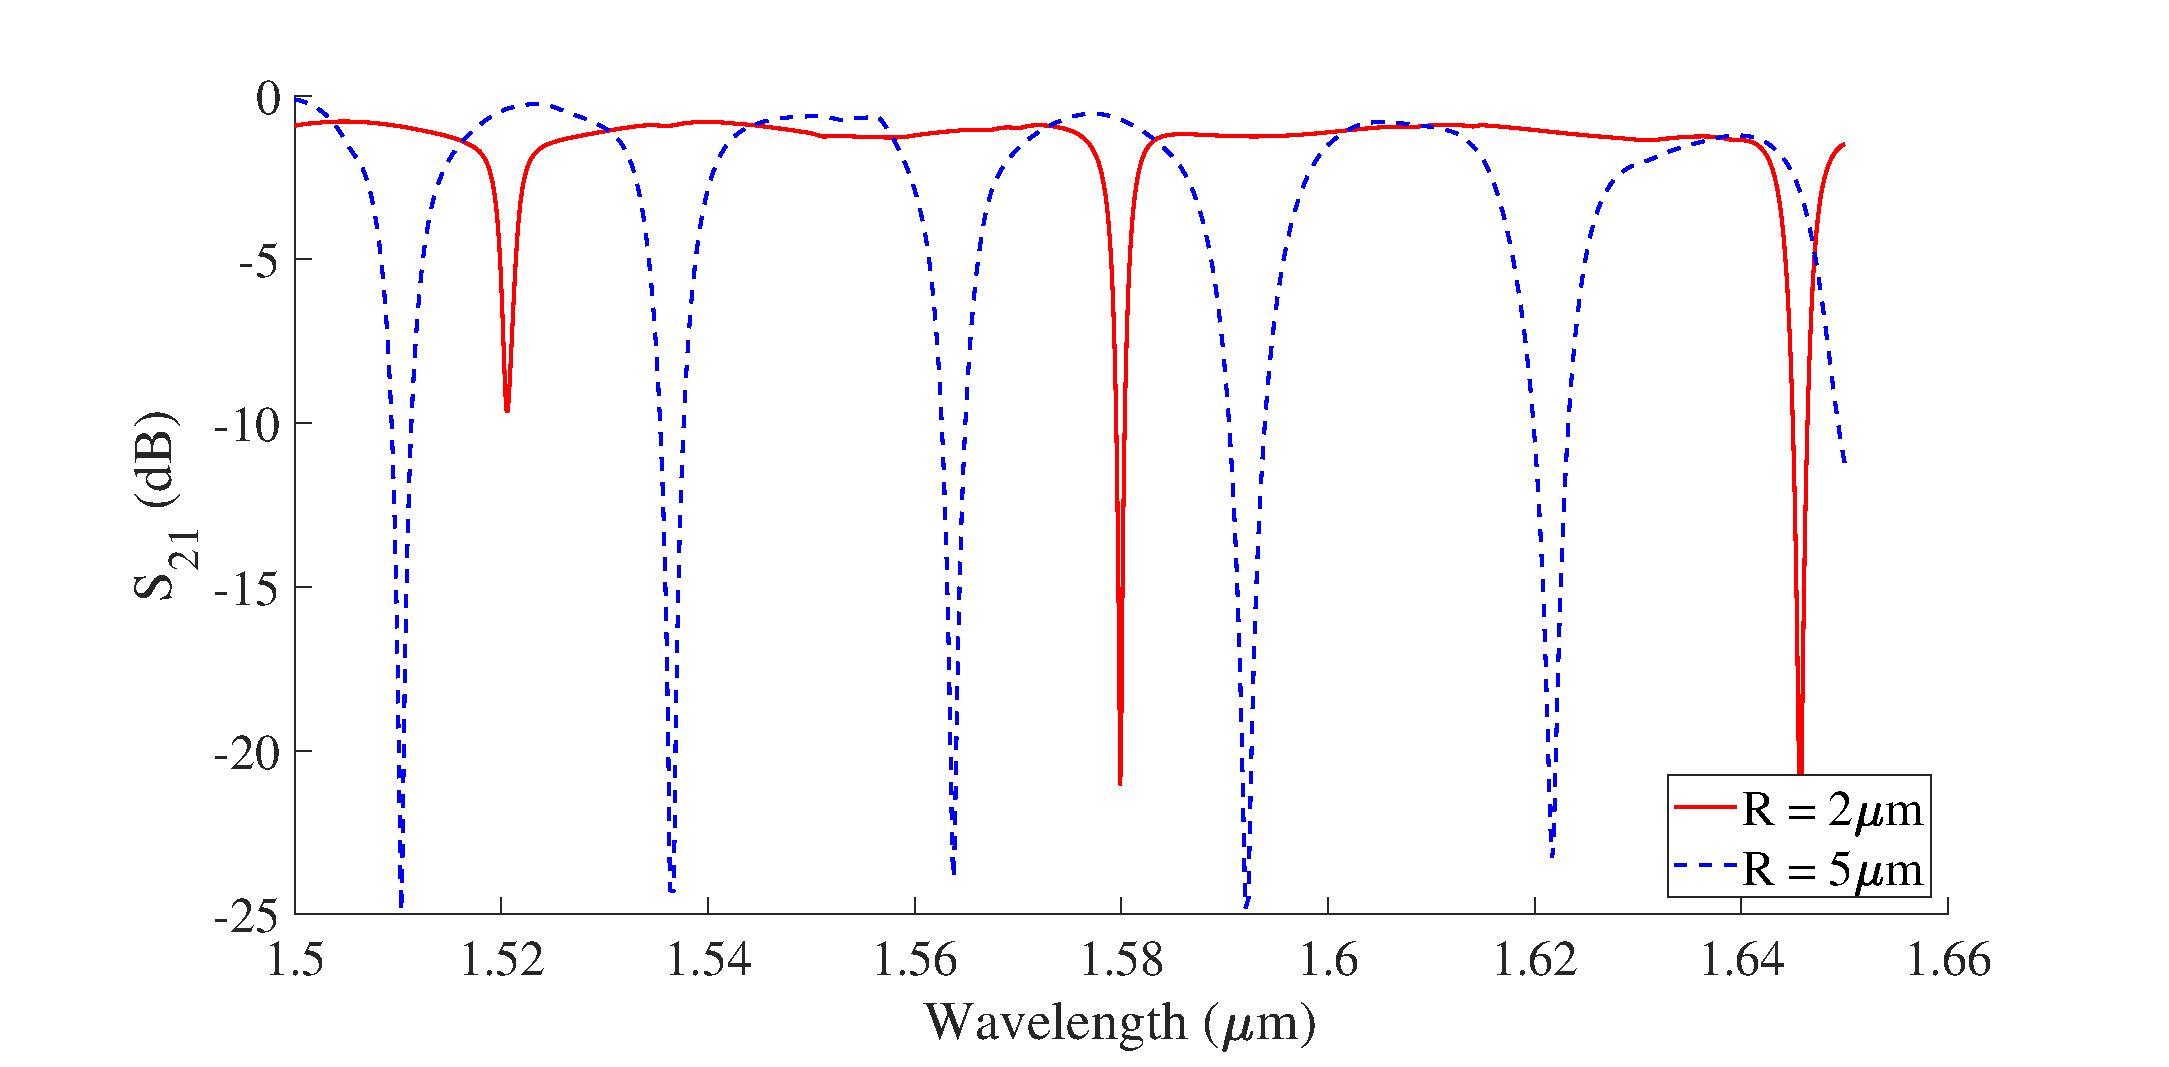
\includegraphics[width=1\textwidth]{hdlw_scatt_param_plot.eps}\vspace{1mm}
	\caption{{Transmission characteristics of HDLW based ring resonator.}}%\vspace{-3mm}
	\label{fig:hdlw_transmission}
\end{figure}

\subsection{Horn-nanoantenna}
Fig.~\ref{fig:hnano_mode_prof} shows that the $\text{SiO}_2$-cladding layer is sandwiched between a metal cap layer and a partly-etched Si layer. The thicknesses of these layers were set at $h_\text{WG}$= 30 nm, $h_\text{Au}$ = 70 nm, and $h_\text{RIB}$ = 100 nm, respectively. The layered structure is taken from~\cite{Yousefi2012} in which the authors have proposed a rectangular patch optical nanoantenna to radiate the optical field from a hybrid plasmonic waveguide.

Fig.~\ref{fig:hnano_mode_prof} and ~\ref{fig:hnano_efield_dist} show the mode profile and the E-field norm distribution of horn-nanoantenna input HP waveguide. It is observed that mode is confined mostly in $\text{SiO}_2$ layer only.

\begin{figure}[!t]
	\centering
	\includegraphics[width=1\textwidth]{hnano_mode_profile.jpg}\vspace{1mm}
	\caption{{Mode profile of horn-nanoantenna input HP waveguide.}}%\vspace{-3mm}
	\label{fig:hnano_mode_prof}
\end{figure}

\begin{figure}[!t]
	\centering
	\includegraphics[width=1\textwidth]{hnano_normE_dist.jpg}\vspace{1mm}
	\caption{{E-field norm distribution of horn-nanoantenna input HP waveguide.}}%\vspace{-3mm}
	\label{fig:hnano_efield_dist}
\end{figure}
